% -*- coding: utf-8 -*-
% Линеаризованная абстракция
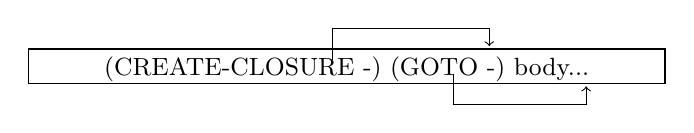
\begin{tikzpicture}
  \tikzstyle{every node}=[font=\small]

  \draw [semithick] (0em, 0em) rectangle (23em, 1.25em);
  \draw (11.5em, 1.33em) node[below]
        {\ic{(CREATE-CLOSURE -) (GOTO -) body...}};

  \draw [->] (11.00em, 0.85em) -- (11.00em, 2em) --
             (16.65em, 2em) -- (16.65em, 1.35em);
  \draw [->] (15.35em, 0.35em) -- (15.35em, -0.75em) --
             (20.15em, -0.75em) -- (20.15em, -0.1em);

\end{tikzpicture}
